\chapter{Write Back}


\begin{wrapfigure}{l}{0.7in}
\caption{Write Back}\label{fig:wb}
\begin{center}
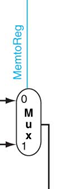
\includegraphics[width=0.5in]{../images/pipeline_writeback.png}
\end{center}
\end{wrapfigure}

\WrapBarrier

\section{Mux}
This stage consists on only one item, a mux to select between the output of memory and the output of the ALU.  The control is the memtoreg control line, see Fig~\ref{fig:wb}.  Since the mux has already been tested it does not need a testbench.  The stage thus has only 3 inputs (2 data and 1 control) and one output, the result.

\section{Pipeline}
You are ready to assemble the pipeline.  The basic pipeline file with all needed wires has been provided.  You need to instantiate your modules and hook the wires up according to Fig~\ref{fig:pipeline}.  Here is my advice on how to do this simply and easily:
\begin{enumerate}
\item Open iFetch and copy the interface (from iFetch to the first `;') then paste it into pipeline after the comment stating `Fetch'.  This will become the instantiation. \label{step:instantiate}
\item Copy all the outputs in the interface again up to the space right after the comment stating `wires from Fetch outputs'.
\item Change all the words outputs to wire in the section for wire instantiation.  You are now ensured that the wires are the right size.
\item Since other modules could use the same names and this could cause conflicts, append \verb1_IFID1 after each wire name you just created to show it came from the IFID buffer.  Make sure you change all the commas to semicolons and put a final semicolon on the last entry.  Later you can use\verb1_IDEX1 for the IDEX buffer, etc.  A few wires will come from a stage without buffering - such as PCSrc from the Mem stage, for which I suggest you use something like \verb1_nbMEM1.  The nb means no buffering and the MEM is for the stage.  I like the stage time it is coming from to be the last thing because when I look in the timing diagram it reads nice to see the stage it comes from as the last (most noticeable) part of the signal name. \label{step:wires}
\item Back in the instantiation part (made in step~\ref{step:instantiate}), change everything before each port name to a `.' and put a pair of parenthesis after the port name.
\item Put \verb1clk_a1 and \verb1reset1 in to the clk and reset ports.
\item Put the appropriate wires you created in step~\ref{step:wires} into the parenthesis of the outputs.
\item The inputs will come from later stages so you will place them when you create the appropriate stage.
\item repeat for the next stage till you finish Write Back.
\end{enumerate}
This may seem tedious at first, but try it and you should find it goes fast and is fairly error-proof.  I would split the stages between the partners in your group.  Decode and Execute are the biggest.  A roughly fair breakdown is one partner does before Fetch and Decode, the other does Execute, Memory, and Write Back.

Note the clock and reset are not shown.  Make sure you use \verb1clk_a1 and not \verb1clk1, the difference being \verb1clk_a1 can also start and stop (while preserving values) the pipeline.  Be careful to pass back signals after the appropriate stage, some signals like exit after the ex-mem buffer.  

Verify by running programs and testing the output.

\begin{figure}
\caption{Full Pipeline.}\label{fig:pipeline}
\begin{center}
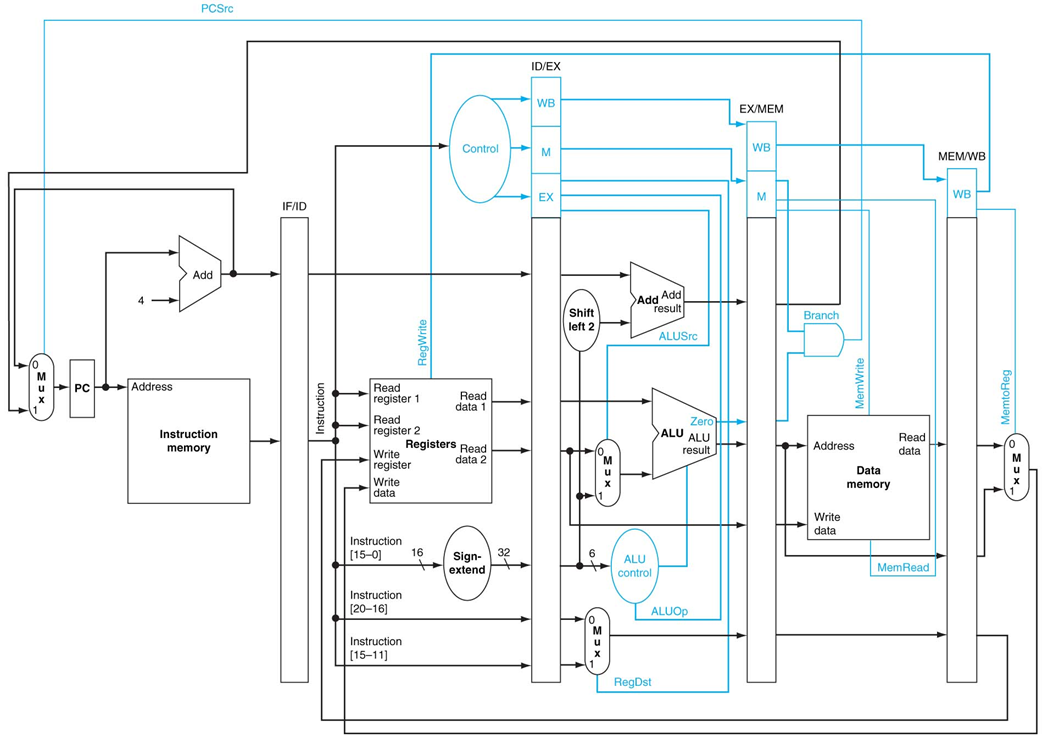
\includegraphics[width=\textwidth]{../images/pipeline_full.png}
\end{center}
\end{figure}

\section{Your Assignment}

You are to:
\begin{enumerate}
\item Create the Writeback stage consisting of one Mux.
\item Integrate all five stages into the file pipeline.v.  Verify with test programs.
\item  Write up a lab report in \LaTeX\ following the lab format in \verb1LabN.tex1 and generate a pdf file.
\item Upload the pdf and all the Verilog files to the course LMS.
\end{enumerate} 